\documentclass{scrartcl}
\usepackage{graphicx}
\usepackage{float}
\usepackage[spanish]{babel}
\usepackage{hyperref} 
\graphicspath{ {img/} }

\title{Diseño de Interfaces}
\subtitle{\large PAMN - Programación de Aplicaciónes Moviles Nativas}
\author{Chamil José Cruz Razeq}

\begin{document}
    \maketitle
    \thispagestyle{empty}
    \newpage
    \tableofcontents
    \newpage

    \section{Introducción}
        Este documento recoge los resultados de la propuesta de tárea diseño de
        interfaces donde se solicita el planteamiento de una aplicación, una 
        primera aproximación a su experiencia de usuario y una muestra del
        posible producto final.

        Todos los documentos están recogidos en el siguiente
        repositorio de \href{https://github.com/chamilstudy/ulpgc_pamn_labs}{GitHub}.
    
    \section{Propuesta}
        Aplicación para la reserva y información sobre áreas recreativas de la
        isla de Gran Canaria. Esta aplicación sería complementaria al servicio
        web del cabildo, donde poder solicitar permisos para acampar o usar las
        instalaciones, recibir información y alertas en tiempo real y facilitar
        información de interés sobre las localizaciones, tanto historicas como
        características.
    \newpage
    \section{Experiencia de Usuario}
        Como elementos comunes de la aplicación tenemos aquellos dirigidos a la
        información o advertencias en tiempo real, tales como la disponibilidad
        de un área o las instalaciones que la componen [Figura 1]. Por otro lado también se
        dispone de un elemento informativo a modo de advertencia para informar
        de circunstancias de emergencia a los usuarios [Figura 2].
        \begin{figure}[H]
            \centerline{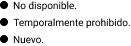
\includegraphics[scale=0.20]{wirestate}}
            \caption{Elemento informativo.}
            \label{fig:wirestate}
        \end{figure}
        \begin{figure}[H]
            \centerline{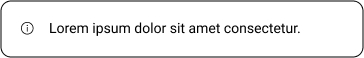
\includegraphics[scale=0.20]{wiredanger}}
            \caption{Advertencia en tiempo real.}
            \label{fig:wiredanger}
        \end{figure}
        Todas las pantallas tienen como características comunes, una cabecera que
        indica donde se encuentra el usuario, y una barra de navegación.
        
        La pantalla principal ofrece un banner con información reciente y la lista
        de áreas recreativas, con posibilidad de ser filtradas y ver información
        sobre el estado del área [Figura 3].
        \begin{figure}[H]
            \centerline{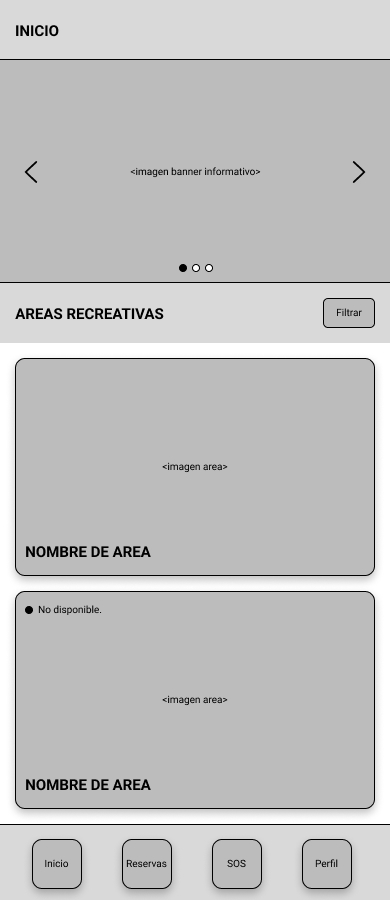
\includegraphics[scale=0.20]{wirehome}}
            \caption{Pantalla Principal}
            \label{fig:wirehome}
        \end{figure}
        La pantalla de área ofrece información relacionada con el espacio recreativo,
        instalaciones, localización y otras actividades, imagenes... y el acceso al
        formulario de solicitud de permisos [Figura 4].
        \begin{figure}[H]
            \centerline{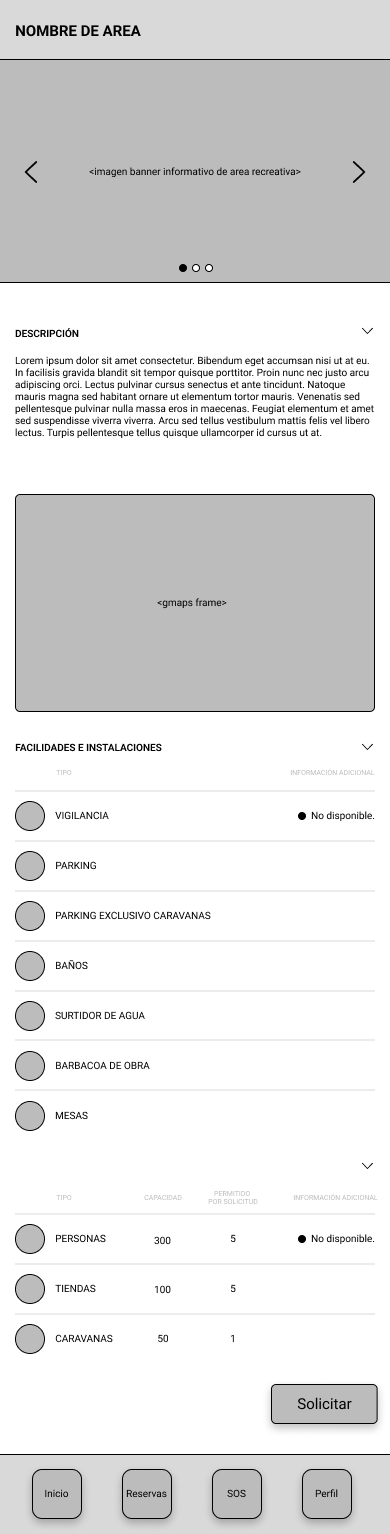
\includegraphics[scale=0.20]{wirearea}}
            \caption{Pantalla de Área Recreativa}
            \label{fig:wireárea}
        \end{figure}
        La [Figura 5] muestra la pantalla de área con sus elementos plegados y una
        advertencia en tiempo real.
        \begin{figure}[H]
            \centerline{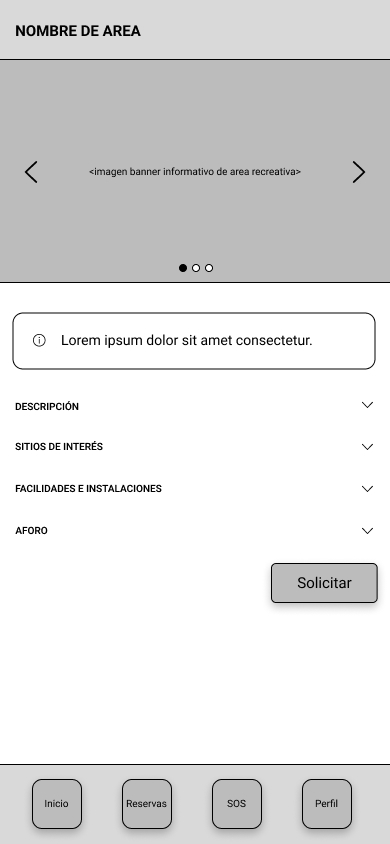
\includegraphics[scale=0.20]{wireareamerged}}
            \caption{Pantalla de Área Recreativa Plegada}
            \label{fig:wireáreamerged}
        \end{figure}
        La pantalla de reservas muestra una lista de las solicitudes realizadas y 
        información sobre la vigencia de la solicitud y elementos reservados [Figura 6].
        \begin{figure}[H]
            \centerline{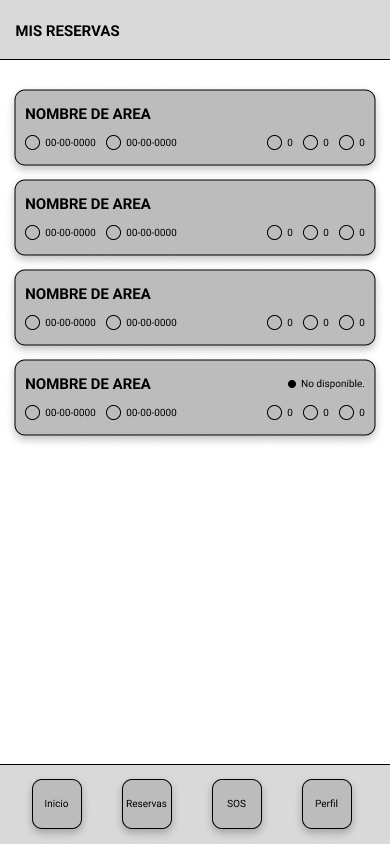
\includegraphics[scale=0.20]{wirebooks}}
            \caption{Pantalla de Reservas}
            \label{fig:wirebooks}
        \end{figure}
        La pantalla de servicios de asistencia ofrece información de contacto de los
        servicios de seguridad y sanitarios [Figura 7].
        \begin{figure}[H]
            \centerline{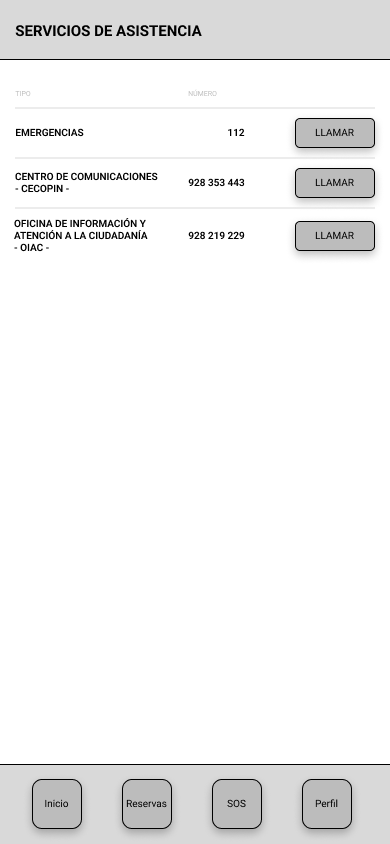
\includegraphics[scale=0.20]{wiresos}}
            \caption{Patalla de Servicios de Asistencia}
            \label{fig:wiresos}
        \end{figure}
    \newpage
    \section{Diseño}
        Utilizando como base el wireframe de pantalla principal [Figura 3] se
        plantea el diseño [Figura 8] como posible interfaz.
        \begin{figure}[H]
            \centerline{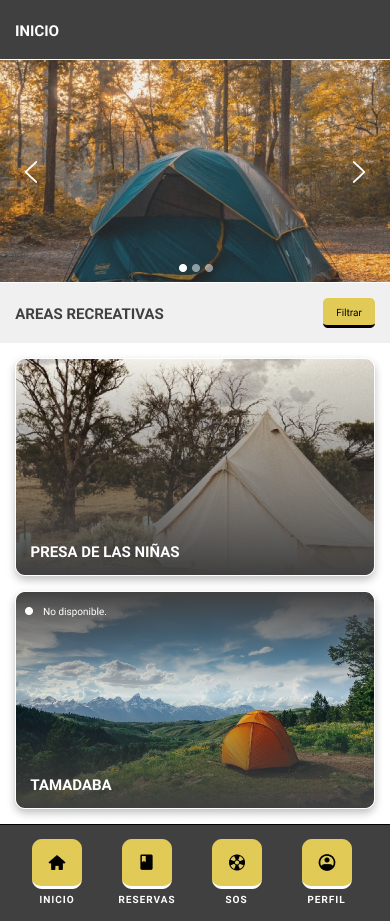
\includegraphics[scale=0.20]{design}}
            \caption{Muestra de Diseño}
            \label{fig:design}
        \end{figure}
\end{document}
